\documentclass{standalone}
\usepackage{tikz}
\usepackage{ctex,siunitx}
\setCJKmainfont{Noto Serif CJK SC}
\usepackage{tkz-euclide}
\usepackage{amsmath}
\usetikzlibrary{patterns, calc,3d}
\usetikzlibrary {decorations.pathmorphing,decorations.pathreplacing,decorations.shapes}
\begin{document}
\small
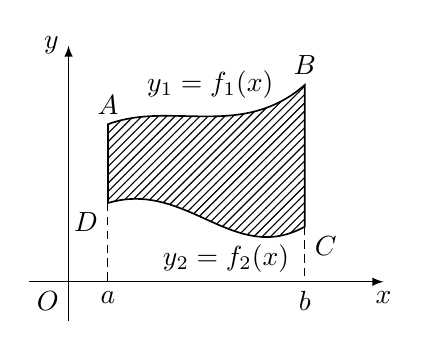
\begin{tikzpicture}[>=latex,scale=1.0]
  \draw[->](-0.5,0)--(4,0)node[below]{$x$};
  \draw[->](0,-0.5)--(0,3.0)node[left]{$y$};
  \node at (0,0)[below left]{$O$};
  \draw[semithick,pattern=north east lines](0.5,2.0)node[above]{$A$}..controls (1.3,2.3)and(2.2,1.8)..(3.0,2.5)node[above]{$B$}--(3.0,0.7)node[below right]{$C$}..controls(2.1,0.2)and(1.5,1.3)..(0.5,1.0)node[below left]{$D$}--cycle;
  \node at (1.8,2.5){$y_1=f_1(x)$};
  \node at (2.0,0.3){$y_2=f_2(x)$};
  \draw[densely dashed](0.5,1.0)--(0.5,0)node[below]{$a$};
  \draw[densely dashed](3.0,0.7)--(3.0,0)node[below]{$b$};
\end{tikzpicture}
\end{document}